\documentclass[journal, a4paper]{IEEEtran}

\usepackage{amsmath,amssymb,amsthm,bm}
\usepackage{mathtools}
\usepackage{enumitem}
\usepackage{graphicx}

% Allow page breaks within multi-line displays (helpful in two-column layouts)
\allowdisplaybreaks

\title{Finite-Dimensional Optimization of a Piecewise-Structured Optimal Driving Policy with Speed-Limit Regimes}
\author{}
\date{\today}

\newcommand{\dd}{\,\mathrm{d}}
\newcommand{\R}{\mathbb{R}}
\newcommand{\argmin}{\operatorname*{arg\,min}}

\begin{document}
\maketitle

\begin{abstract}
We study a simplified longitudinal driving model with a power-limited engine, quadratic aerodynamic drag, linear rolling/drivetrain losses, an added constant parasitic resistance, and optional braking.
A driver minimizes a sum of time cost, fuel cost, and expected speeding fines along a road with a baseline speed-limit regime and a reduced-limit zone on $x\in[0,L]$.
A Pontryagin Maximum Principle (PMP) analysis implies that optimal extremals are concatenations of bang--bang propulsion/braking arcs and throttle-singular cruise arcs.
Motivated by this structure, we restrict to a five-stage trajectory family:
(i) optimal constant-speed cruising outside the zone,
(ii) deceleration to the optimal zone cruise speed using either coasting or full braking,
(iii) optimal constant-speed cruising inside the zone,
(iv) maximum acceleration back to the outside optimal cruise speed, and
(v) optimal constant-speed cruising outside the zone.
Within this family, the problem reduces to a finite-dimensional comparison of four discrete placement options for the deceleration and acceleration arcs relative to $x=0$ and $x=L$, with explicit quadratures for distances and costs.
We also provide a simple parameter identification procedure using sparse fuel-consumption and coasting-deceleration measurements, yielding a smooth fuel-consumption curve consistent with data.
\end{abstract}

\section{Model}\label{sec:model}

\subsection{Dynamics with a constant parasitic term}
Let $x(t)$ be position and $v(t)\ge 0$ speed. Controls are throttle $u(t)\in[0,1]$ and braking command $b(t)\in[0,1]$.
We model propulsive force as power-limited,
\begin{align}
F_{\mathrm{engine}}(t) &= \frac{P_{\max}\,u(t)}{v(t)+v_0},
\end{align}
aerodynamic drag,
\begin{align}
F_{\mathrm{drag}}(v) &= C_d v^2,
\end{align}
linear rolling/drivetrain resistance,
\begin{align}
F_{\mathrm{roll}}(v) &= m\,\mu_{\mathrm{roll}}\,v,
\end{align}
a constant parasitic resistance (e.g.\ accessory loads and Coulomb-like drivetrain losses),
\begin{align}
F_{0} &= m\,\mu_0,
\end{align}
and braking force
\begin{align}
F_{\mathrm{brake}}(t) &= m\,a_{\mathrm{brake}}\,b(t).
\end{align}
The longitudinal dynamics are
\begin{align}
\dot{x} &= v, \label{eq:xdot}\\
\dot{v} &= \frac{1}{m}\Big(
  F_{\mathrm{engine}}-F_{\mathrm{drag}}-F_{\mathrm{roll}}-F_{0}-F_{\mathrm{brake}}
\Big). \label{eq:vdot}
\end{align}

It is convenient to introduce constants
\begin{align}
A &:= \frac{P_{\max}}{m}, & B &:= \frac{C_d}{m}, \notag\\
\mu &:= \mu_{\mathrm{roll}}, & a &:= a_{\mathrm{brake}}.
\end{align}
Then \eqref{eq:vdot} becomes
\begin{align}
\dot{v}
  &= A\frac{u}{v+v_0} - Bv^2 - \mu v - \mu_0 - a b.
\label{eq:vdot_compact}
\end{align}

\subsection{Running cost: time, fuel, expected fines}
Let $C_t>0$ be the monetary cost rate of time (money per unit time).

\paragraph{Fuel model}
Let $f(t)$ denote fuel consumed (in fuel units, e.g., liters), and assume an affine fuel consumption rate in throttle,
\begin{align}
\dot{f}(t)=\gamma_u\,u(t)+\gamma_0
\qquad\text{(fuel units/time)},
\label{eq:fuel_affine}
\end{align}
where $\gamma_u\ge 0$ and $\gamma_0\ge 0$ are model parameters.
If $c_f$ is the fuel price (money per fuel unit), then the fuel \emph{cost rate} (money per unit time) is
\begin{align}
\ell_{\mathrm{fuel}}(u)
  &= c_f \bigl(\gamma_u u+\gamma_0\bigr) \notag\\
  &:= \alpha u + \beta, \notag\\
\alpha &:=\gamma_u c_f, \qquad
\beta :=\gamma_0 c_f.
\label{eq:fuel_rate}
\end{align}

\paragraph{Speed-limit regimes and expected fines}
There are two regimes:
\begin{itemize}[leftmargin=2em]
\item \emph{Outside} the zone ($x\notin[0,L]$): speed limit $v_{\mathrm{lim},1}$ and ``higher speeding'' threshold $v_{\max,1}$.
\item \emph{Inside} the zone ($x\in[0,L]$): speed limit $v_{\mathrm{lim},2} < v_{\mathrm{lim},1}$ and threshold $v_{\max,2}$.
\end{itemize}
A driver speeding above the applicable limit may incur an expected fine. To keep the objective additive in time, we model this via an \emph{expected fine rate} (money per unit time). Let $\lambda_{\mathrm{out}},\lambda_{\mathrm{in}}\ge 0$ be enforcement intensities (per unit time), $p_L\in[0,1]$ a probability factor, and $P_{\mathrm{low}}<P_{\mathrm{high}}$ the low/high fine amounts. Define, for each regime $\mathrm{reg}\in\{\mathrm{out},\mathrm{in}\}$,
\begin{align}
\phi_{\mathrm{reg}}(v)=
\begin{cases}
0, & v\le v_{\mathrm{lim},\mathrm{reg}},\\
p_L P_{\mathrm{low}}\,\lambda_{\mathrm{reg}},
  & v_{\mathrm{lim},\mathrm{reg}}< v\le v_{\max,\mathrm{reg}},\\
p_L P_{\mathrm{high}}\,\lambda_{\mathrm{reg}},
  & v> v_{\max,\mathrm{reg}}.
\end{cases}
\label{eq:fine_rate}
\end{align}
Here $(v_{\mathrm{lim},\mathrm{out}},v_{\max,\mathrm{out}})=(v_{\mathrm{lim},1},v_{\max,1})$ and $(v_{\mathrm{lim},\mathrm{in}},v_{\max,\mathrm{in}})=(v_{\mathrm{lim},2},v_{\max,2})$.

\paragraph{Total running cost rate}
In regime $\mathrm{reg}\in\{\mathrm{out},\mathrm{in}\}$ we take
\begin{align}
\ell_{\mathrm{reg}}(v,u)
  &= C_t + (\alpha u+\beta) + \phi_{\mathrm{reg}}(v).
\label{eq:running_cost}
\end{align}

\paragraph{Total cost functional}
For a trajectory segment with regime determined by $x(t)$, we minimize
\begin{align}
J = \int_0^T \ell(x(t),v(t),u(t))\,\dd t,
\end{align}
where $\ell=\ell_{\mathrm{out}}$ when $x\notin[0,L]$ and $\ell=\ell_{\mathrm{in}}$ when $x\in[0,L]$.

\section{Calibration from sparse measurements}\label{sec:calibration}
This section shows how the additional constant resistance $\mu_0$ enables a smooth fit to sparse measurements of fuel consumption and coasting deceleration.

\subsection{Fuel per distance under steady cruising}
At constant speed (no braking), $\dot v=0$ in \eqref{eq:vdot_compact} implies the steady-cruise throttle
\begin{align}
u_{\mathrm{cruise}}(v)
&= \frac{(v+v_0)\bigl(Bv^2+\mu v+\mu_0\bigr)}{A}.
\label{eq:u_cruise}
\end{align}
Let $V$ be speed in km/h and $v=V/3.6$ in m/s. Since $\dot f$ is in L/h, fuel consumption in liters per 100 km is
\begin{align}
\mathrm{FC}_{100}(V)
&:= \bigl(\gamma_u u_{\mathrm{cruise}}(V)+\gamma_0\bigr)\frac{100}{V},
\qquad V>0.
\label{eq:FC100_def}
\end{align}
The term $\gamma_0$ contributes a $1/V$ component to $\mathrm{FC}_{100}$, while the power-limited engine model introduces higher-order dependence through \eqref{eq:u_cruise}.

\subsection{Using coasting deceleration to fix $(B,\mu,\mu_0)$}
With $u=0$ and $b=0$ (coasting), \eqref{eq:vdot_compact} gives
\begin{align}
\dot v = -(Bv^2+\mu v+\mu_0).
\label{eq:vdot_coast_cal}
\end{align}
At a given speed $v$, the instantaneous coasting deceleration magnitude is therefore
\begin{align}
a_{\mathrm{coast}}(v)=Bv^2+\mu v+\mu_0.
\label{eq:acoast}
\end{align}

\subsection{Numerical parameter set consistent with data}
We impose the following measurements (with $\pm 0.5$ L/100 km uncertainty for fuel points):
\begin{itemize}[leftmargin=2em]
\item Standstill consumption: $\gamma_0=0.6$ L/h.
\item $\mathrm{FC}_{100}(130)=6.5$ L/100 km, $\mathrm{FC}_{100}(80)=5.0$ L/100 km, $\mathrm{FC}_{100}(9)=10.0$ L/100 km.
\item Coasting at 130 km/h loses 10 km/h in 3--6 seconds, corresponding to
\[
a_{\mathrm{coast}}(v_{130})\in[0.46,0.93]\ \mathrm{m/s^2},\quad v_{130}=130/3.6,
\]
and we use the midpoint $a_{\mathrm{coast}}(v_{130})\approx 0.65$ m/s$^2$ for calibration.
\end{itemize}
We fix $v_0=1$ m/s and $P_{\max}=110$ kW, and keep the original linear throttle fuel law with $\gamma_u=19$ L/h.
Solving the resulting system for $(B,\mu,\mu_0)$ and the identifiable ratio $\gamma_u/A$ yields
\begin{align}
B &= 1.4726\times 10^{-4}\ \mathrm{m^{-1}},\notag\\
\mu &= 5.8166\times 10^{-3}\ \mathrm{s^{-1}},\notag\\
\mu_0 &= 2.4793\times 10^{-1}\ \mathrm{m/s^2},\notag\\
\frac{\gamma_u}{A} &= 3.25426\times 10^{-1}\ \mathrm{\frac{L/h}{m/s^2}}.
\label{eq:calibrated_accel_params}
\end{align}
Since $A=P_{\max}/m$, fixing $\gamma_u$ and $P_{\max}$ determines $m$ from $\gamma_u/A$:
\begin{align}
A \approx 58.39\ \mathrm{m/s^2},\qquad m\approx \frac{P_{\max}}{A}\approx 1.884\times 10^3\ \mathrm{kg}.
\label{eq:mass_from_ratio}
\end{align}
In force-form parameters this corresponds to
\begin{align}
C_d &= mB \approx 2.774\times 10^{-1}\ \mathrm{\frac{N}{(m/s)^2}},\notag\\
m\mu_{\mathrm{roll}} &= m\mu \approx 1.096\times 10^{1}\ \mathrm{\frac{N}{m/s}},\notag\\
F_0 &= m\mu_0 \approx 4.67\times 10^{2}\ \mathrm{N}.
\label{eq:calibrated_force_params}
\end{align}

\begin{figure}[!t]
  \centering
  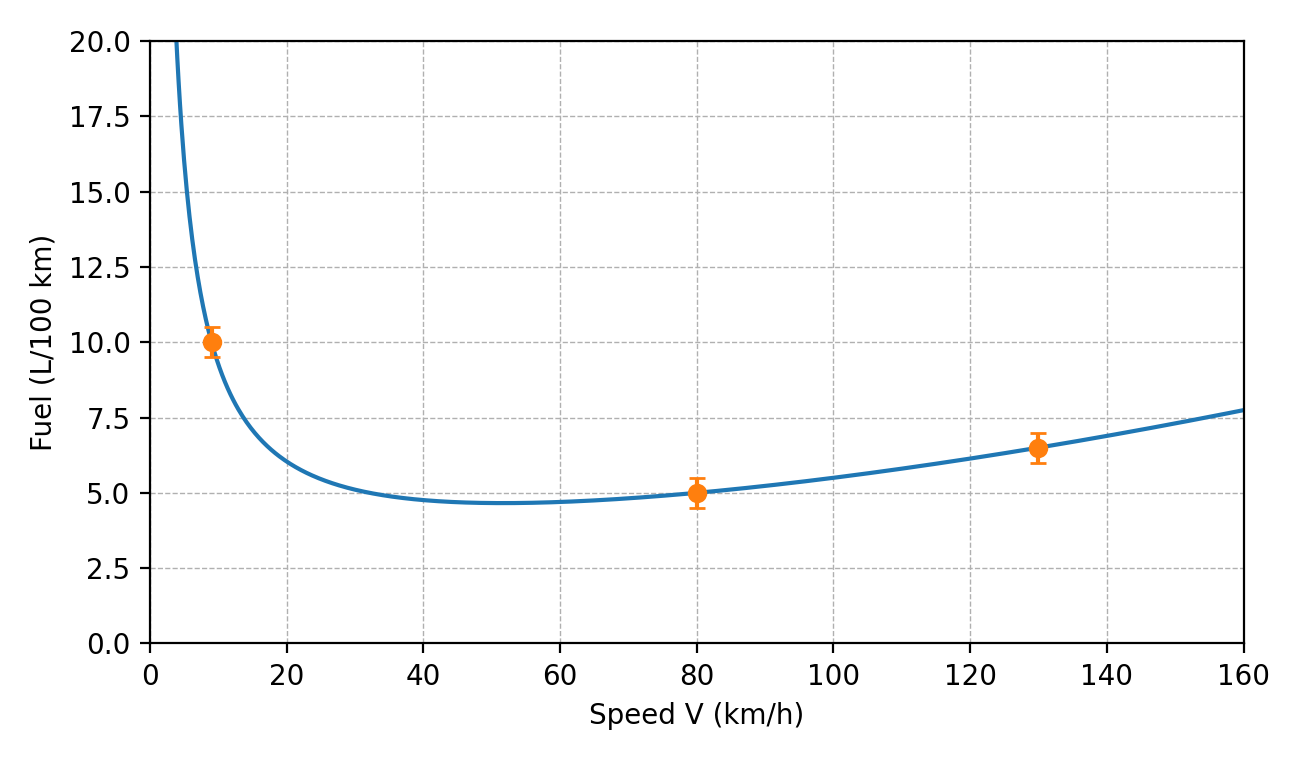
\includegraphics[width=\columnwidth]{fuel_curve.png}
  \caption{Calibrated steady-cruise fuel consumption $\mathrm{FC}_{100}(V)$ from \eqref{eq:FC100_def} using \eqref{eq:calibrated_accel_params}, with measurement points and $\pm 0.5$ L/100 km error bars at $V\in\{9,80,130\}$ km/h. The curve is smooth by construction, coming from the resistance model $Bv^2+\mu v+\mu_0$ and the power-limited propulsion model.}
  \label{fig:fuel_curve}
\end{figure}

\section{Constant-Speed Cruising and Optimal Cruise Speeds}\label{sec:cruise_opt}
A key ingredient is the \emph{optimal constant-speed motion} in each regime. On a constant-speed segment, $\dot v=0$ and we take $b=0$, so \eqref{eq:vdot_compact} yields the steady throttle \eqref{eq:u_cruise}. This is feasible if $0\le u_{\mathrm{cruise}}(v)\le 1$.

\subsection{Cost per distance for cruising}
On a constant-speed segment, $\dot x=v$ and the cost per distance is
\begin{align}
g_{\mathrm{reg}}(v)
  &:= \frac{\ell_{\mathrm{reg}}(v,u_{\mathrm{cruise}}(v))}{v} \notag\\
  &= \frac{C_t+\beta+\alpha u_{\mathrm{cruise}}(v)+\phi_{\mathrm{reg}}(v)}{v}.
\label{eq:g_reg}
\end{align}
The \emph{optimal cruising speeds} are defined by
\begin{align}
v_{\mathrm{out}}
  &\in \argmin_{\substack{v\ge 0\\ u_{\mathrm{cruise}}(v)\in[0,1]}}
      g_{\mathrm{out}}(v), \notag\\
v_{\mathrm{in}}
  &\in \argmin_{\substack{v\ge 0\\ u_{\mathrm{cruise}}(v)\in[0,1]}}
      g_{\mathrm{in}}(v).
\label{eq:v_opt_defs}
\end{align}

\subsection{Stationary condition (within a speed band)}
Within any interval of speeds where $\phi_{\mathrm{reg}}(v)$ is constant (i.e.\ between thresholds), differentiability holds and a stationary point satisfies
\begin{align}
\frac{\dd}{\dd v}\Big(\frac{k_{\mathrm{reg}}(v)}{v}\Big)=0
\quad\Longleftrightarrow\quad
v k'_{\mathrm{reg}}(v)-k_{\mathrm{reg}}(v)=0,
\label{eq:stationary_general}
\end{align}
where
\begin{align}
k_{\mathrm{reg}}(v)
  &:= C_t+\beta+\alpha u_{\mathrm{cruise}}(v)+\phi_{\mathrm{reg}}(v).
\end{align}
Since $\phi'_{\mathrm{reg}}(v)=0$ within a band, \eqref{eq:stationary_general} becomes
\begin{align}
v\,\alpha\,u'_{\mathrm{cruise}}(v)
  &= C_t+\beta+\alpha u_{\mathrm{cruise}}(v)+\phi_{\mathrm{reg}}.
\label{eq:stationary_band}
\end{align}
Expanding \eqref{eq:u_cruise} gives
\begin{align}
u_{\mathrm{cruise}}(v)
&=\frac{1}{A}\Big(
  Bv^3+(\mu+Bv_0)v^2+(\mu_0+\mu v_0)v+\mu_0 v_0
\Big), \label{eq:u_cruise_poly}\\
u'_{\mathrm{cruise}}(v)
&=\frac{1}{A}\Big(
  3Bv^2+2(\mu+Bv_0)v+(\mu_0+\mu v_0)
\Big).
\label{eq:u_cruise_deriv}
\end{align}
Because $\phi_{\mathrm{reg}}$ is piecewise constant with jumps at $v=v_{\mathrm{lim},\mathrm{reg}}$ and $v=v_{\max,\mathrm{reg}}$, the global minimizer of $g_{\mathrm{reg}}$ may occur either at an interior stationary point in a band or at these thresholds; one compares all feasible candidates.

\section{Pontryagin Maximum Principle and Admissible Arc Types}\label{sec:PMP_arcs}

This section explains why the five-stage family considered later is not ad hoc: it is directly motivated by the structure of optimal controls implied by the Pontryagin Maximum Principle (PMP) for our model.

\subsection{Optimal control problem and Hamiltonian}
We consider the problem of minimizing the integral cost
\begin{align}
J=\int_0^T \ell(x(t),v(t),u(t))\,\dd t,
\end{align}
subject to the dynamics \eqref{eq:xdot}--\eqref{eq:vdot_compact} and bounds $u(t)\in[0,1]$, $b(t)\in[0,1]$, with $v(t)\ge 0$.
The running cost depends on the active regime through \eqref{eq:running_cost}:
$\ell=\ell_{\mathrm{out}}$ for $x\notin[0,L]$ and $\ell=\ell_{\mathrm{in}}$ for $x\in[0,L]$.

Let $\psi_x(t)$ and $\psi_v(t)$ be the costates. The Hamiltonian in regime $\mathrm{reg}\in\{\mathrm{out},\mathrm{in}\}$ is
\begin{align}
H_{\mathrm{reg}}
=& \ell_{\mathrm{reg}}(v,u)\nonumber
   + \psi_x\,v\\
&   + \psi_v\Big(A\frac{u}{v+v_0}-Bv^2-\mu v-\mu_0-a b\Big).
\label{eq:Hamiltonian}
\end{align}

\subsection{Costate equations and regime discontinuities}
Within a region where the regime is fixed (so $\ell_{\mathrm{reg}}$ is fixed as a function of $(v,u)$), the PMP costate equations are
\begin{align}
\dot\psi_x &= -\frac{\partial H_{\mathrm{reg}}}{\partial x},
\label{eq:psix_dot}\\
\dot\psi_v &= -\frac{\partial H_{\mathrm{reg}}}{\partial v}.
\label{eq:psiv_dot}
\end{align}
In our model, the $x$-dependence of $H_{\mathrm{reg}}$ arises only through regime selection and the expected-fine term $\phi_{\mathrm{reg}}(v)$.
Thus, \emph{away from the regime boundaries} $x=0$ and $x=L$ we have $\partial H_{\mathrm{reg}}/\partial x=0$, hence
\begin{align}
\dot\psi_x =0
\quad\text{(a.e.\ on each regime region).}
\label{eq:psix_piecewise_constant}
\end{align}
At $x=0$ and $x=L$ the running cost changes discontinuously (because $\phi_{\mathrm{reg}}$ changes), and hybrid PMP allows corresponding \emph{corner/jump conditions}. Informally, $\psi_x$ can jump at $x\in\{0,L\}$, while the states remain continuous. This observation is one reason why optimal switching is naturally aligned with the regime boundaries.

Differentiating \eqref{eq:Hamiltonian} w.r.t.\ $v$ gives, for fixed regime,
\begin{align}
\dot\psi_v
=& -\frac{\partial \ell_{\mathrm{reg}}}{\partial v}
   -\psi_x\nonumber\\
 &  -\psi_v\frac{\partial}{\partial v}\Big(A\frac{u}{v+v_0}-Bv^2-\mu v-a b-\mu_0\Big)\notag\\
=& -\phi'_{\mathrm{reg}}(v)
   -\psi_x
   +\psi_v\Big(A\frac{u}{(v+v_0)^2}+2Bv+\mu\Big).
\label{eq:psiv_explicit}
\end{align}
Because $\phi_{\mathrm{reg}}(v)$ is \emph{piecewise constant} in $v$ (with thresholds at $v=v_{\mathrm{lim},\mathrm{reg}}$ and $v=v_{\max,\mathrm{reg}}$), we have $\phi'_{\mathrm{reg}}(v)=0$ for almost all $v$, with possible corner effects when a trajectory hits a threshold exactly. These speed thresholds therefore form another set of natural candidate locations for switching behavior.

\subsection{Bang--bang structure from affine dependence on controls}
Crucially, $H_{\mathrm{reg}}$ is \emph{affine} (linear) in $u$ and in $b$. Collecting the $u$-terms in \eqref{eq:Hamiltonian} yields
\begin{align}
H_{\mathrm{reg}}
= \dots + u\Big(\alpha + \psi_v\frac{A}{v+v_0}\Big) \;-\; \psi_v a b.
\end{align}
Define the switching functions
\begin{align}
\sigma_u(t) &:= \alpha + \psi_v(t)\frac{A}{v(t)+v_0},
\label{eq:sigma_u}\\
\sigma_b(t) &:= -a\,\psi_v(t).
\label{eq:sigma_b}
\end{align}
Minimizing $H_{\mathrm{reg}}$ over $u\in[0,1]$ and $b\in[0,1]$ gives the pointwise optimal controls
\begin{align}
u^\star(t) &=
\begin{cases}
0, & \sigma_u(t)>0,\\
1, & \sigma_u(t)<0,\\
\text{singular}, & \sigma_u(t)=0,
\end{cases}
\label{eq:u_bangbang}\\
b^\star(t) &=
\begin{cases}
0, & \psi_v(t)<0,\\
1, & \psi_v(t)>0,\\
\text{singular}, & \psi_v(t)=0.
\end{cases}
\label{eq:b_bangbang}
\end{align}
Therefore, \emph{except on singular arcs} where $\sigma_u\equiv 0$ (or $\psi_v\equiv 0$), optimal controls are bang--bang:
\begin{itemize}[leftmargin=2em]
\item \textbf{Coasting:} $u=0$ (and typically $b=0$);
\item \textbf{Maximum acceleration:} $u=1$, $b=0$;
\item \textbf{Full braking:} $u=0$, $b=1$.
\end{itemize}
This is the fundamental PMP justification for restricting to the finite set of arc types used later.

\subsection{Singular throttle arcs and constant-speed cruising}\label{sec:singular_cruise}
Because the Hamiltonian \eqref{eq:Hamiltonian} is affine in the throttle $u$, any optimal solution with an \emph{interior} throttle value $u^\star(t)\in(0,1)$ over a nontrivial time interval must be a \emph{singular arc} in the PMP sense. Concretely, the minimizer of an affine function over the interval $[0,1]$ lies at an endpoint unless the coefficient of $u$ vanishes. Writing the $u$-dependence of $H_{\mathrm{reg}}$ explicitly,
\begin{align}
H_{\mathrm{reg}}
= \cdots + u\Big(\alpha+\psi_v\frac{A}{v+v_0}\Big),
\end{align}
we obtain the switching function $\sigma_u$ in \eqref{eq:sigma_u}. Therefore,
\begin{align}
u^\star(t)&\in(0,1)\nonumber
\ \text{on an interval}
\quad\Longrightarrow\quad\\
\sigma_u(t)&\equiv 0
\ \text{on that interval}.
\label{eq:interior_implies_singular}
\end{align}
Equivalently, on any throttle-singular interval,
\begin{align}
\sigma_u=0
\quad\Longleftrightarrow\quad
\psi_v = -\alpha\,\frac{v+v_0}{A}.
\label{eq:singular_relation_repeat}
\end{align}

\paragraph{Constant speed requires interior throttle}
A constant-speed segment with $v(t)\equiv \bar v>0$ and no braking ($b=0$) must satisfy $\dot v=0$. From \eqref{eq:vdot_compact} this imposes
\begin{align}
0 &= A\frac{u}{\bar v+v_0}-B\bar v^2-\mu \bar v \nonumber \\
\quad&\Longrightarrow\quad
u = u_{\mathrm{cruise}}(\bar v)
=\frac{(\bar v+v_0)(B\bar v^2+\mu \bar v+\mu_0)}{A}.
\end{align}
which is generally an interior value $u_{\mathrm{cruise}}(\bar v)\in(0,1)$ for feasible cruising speeds.
By \eqref{eq:interior_implies_singular}, such a constant-speed segment is necessarily a \emph{throttle-singular arc} of the PMP extremals (unless it lies exactly at a boundary value $u=0$ or $u=1$, which would correspond to degenerate cases such as coasting at $\bar v=0$ or saturating the actuator).

\paragraph{Conversely: singular arcs naturally realize constant-speed motion}
On a throttle-singular arc, $\sigma_u\equiv 0$ and the PMP additionally requires consistency of this condition (classically $\dot\sigma_u=0$ along the arc). In the present model, a robust and practically relevant way to satisfy this consistency is to keep the speed constant, $v(t)\equiv \bar v$, and select the interior throttle $u=u_{\mathrm{cruise}}(\bar v)$ so that $\dot v=0$.
Thus, constant-speed cruising appears as the canonical realization of a throttle-singular extremal arc in this problem class.

\paragraph{Admissibility and ``always available'' cruise segments}
Importantly, for any chosen cruise speed $\bar v$ such that $u_{\mathrm{cruise}}(\bar v)\in[0,1]$, the pair
\begin{align}
v(t)\equiv \bar v,\qquad
u(t)\equiv u_{\mathrm{cruise}}(\bar v),\qquad
b(t)\equiv 0
\end{align}
is dynamically feasible and satisfies the stationarity requirement of the Hamiltonian with respect to $u$ (since it corresponds to an interior control and hence enforces $\sigma_u\equiv 0$).
Therefore constant-velocity segments are always \emph{admissible} building blocks for extremals, and whenever the optimal policy chooses to maintain a speed rather than accelerate/decelerate, it must do so on such a throttle-singular cruise arc.

\paragraph{Remark (leaving the singular arc)}
A cruise (singular) arc can be concatenated with bang--bang arcs at any position/time as long as the junction conditions are satisfied (continuity of states and, away from regime boundaries, of costates) and the switching functions are consistent with the control change. In our finite-dimensional family this freedom is represented by allowing the start/end positions of constant-speed segments to vary, while the principal non-smooth candidates are tied to the regime and speed-threshold discontinuities discussed in Section~\ref{sec:PMP_arcs}.

\subsection{Where can switches occur?}
PMP suggests the following set of \emph{candidate switching events}:
\begin{enumerate}[leftmargin=2em]
\item \textbf{Switching-function zeros:} times where $\sigma_u(t)=0$ (throttle switch) or $\psi_v(t)=0$ (brake switch), which mark transitions among $u=0$, $u=1$, and singular cruise, and among $b=0$ and $b=1$.
\item \textbf{Regime boundaries in space:} $x=0$ and $x=L$, where $\ell(x,\cdot)$ changes discontinuously because the applicable speed limit and fine thresholds change. Hybrid PMP allows a corner condition here (in particular, $\psi_x$ can jump), making these points natural locations for switching.
\item \textbf{Speed-threshold discontinuities:} $v=v_{\mathrm{lim},\mathrm{reg}}$ and $v=v_{\max,\mathrm{reg}}$, where $\phi_{\mathrm{reg}}(v)$ jumps. If an optimal trajectory chooses to ``ride'' a threshold (e.g.\ travel exactly at the limit), these are again natural junction points.
\end{enumerate}
These observations provide the conceptual basis for the five-stage Ansatz in Section~\ref{sec:placement_costs}: constant-speed singular cruise arcs connected by bang--bang deceleration/acceleration arcs, with switching positions naturally tied to $x=0$ and $x=L$ (and, when relevant, to the speed thresholds).

\section{Five-Stage Trajectory Ansatz and Switching Positions}\label{sec:ansatz}

Motivated by the PMP arc structure (bang--bang propulsion/braking with possible throttle-singular cruise arcs), we restrict attention to the same five \emph{arc types} as before:
\begin{enumerate}[label=\arabic*)]
\item Cruise at constant speed $v_{\mathrm{out}}$ (optimal outside).
\item Decelerate from $v_{\mathrm{out}}$ to $v_{\mathrm{in}}$ with $u=0$, using either coasting ($b=0$) or full braking ($b=1$).
\item Cruise at constant speed $v_{\mathrm{in}}$ (optimal inside).
\item Accelerate from $v_{\mathrm{in}}$ to $v_{\mathrm{out}}$ with maximum propulsion $u=1$ (and $b=0$).
\item Cruise at constant speed $v_{\mathrm{out}}$ (optimal outside).
\end{enumerate}
However, the \emph{switching locations} between these arcs should not be discretized a priori to lie exactly at the regime boundaries $x=0$ and $x=L$.
Because the stage-2 and stage-4 dynamics are autonomous in $v$ (they depend on $v$ but not explicitly on $x$), a deceleration or acceleration arc can straddle a regime boundary; the only quantity that matters for the split between ``outside'' and ``inside'' cost accounting is the \emph{speed at the boundary crossing}.
This yields a continuous, finite-dimensional parametrization by boundary-crossing speeds, replacing the earlier four discrete placement options.

\subsection{Boundary-speed parametrization of switching positions}
Let $v_{\mathrm{out}}$ and $v_{\mathrm{in}}$ be the regime-optimal cruise speeds defined in \eqref{eq:v_opt_defs}, and fix a deceleration variant $\mathrm{dec}\in\{\mathrm{coast},\mathrm{brake}\}$.

\paragraph{Entry boundary $x=0$.}
We allow the deceleration arc to begin at some point $x_{12}<0$ while cruising at $v_{\mathrm{out}}$, cross the regime boundary $x=0$ at speed
\begin{align}
v_b := v(0)\in[v_{\mathrm{in}},v_{\mathrm{out}}],
\end{align}
and then complete the deceleration inside the zone to reach $v_{\mathrm{in}}$ at $x_{23}>0$.
Thus $v_b$ parameterizes where the trajectory \emph{departs} from the outside cruise and where it \emph{arrives} at the inside cruise.
With the deceleration dynamics (stage 2) defining $\dd x/\dd v = -v/R_{\mathrm{dec}}(v)$ (see Section~\ref{sec:arc_quadratures}),
the distances of the outside and inside portions of the deceleration arc are
\begin{align}
D^{\mathrm{out}}_{\mathrm{dec}}(v_b)
  &= \int_{v_b}^{v_{\mathrm{out}}}\frac{v}{R_{\mathrm{dec}}(v)}\,\dd v,
\nonumber\\
D^{\mathrm{in}}_{\mathrm{dec}}(v_b)
  &= \int_{v_{\mathrm{in}}}^{v_b}\frac{v}{R_{\mathrm{dec}}(v)}\,\dd v,
\label{eq:dec_split_distances}
\end{align}
so the start and end positions of stage~2 are
\begin{align}
x_{12}=-D^{\mathrm{out}}_{\mathrm{dec}}(v_b),
\qquad
x_{23}= D^{\mathrm{in}}_{\mathrm{dec}}(v_b).
\label{eq:dec_split_positions}
\end{align}

\paragraph{Exit boundary $x=L$.}
Similarly, allow the acceleration arc to start inside the zone at some $x_{34}<L$, cross $x=L$ at speed
\begin{align}
v_c := v(L)\in[v_{\mathrm{in}},v_{\mathrm{out}}],
\end{align}
and complete outside to reach $v_{\mathrm{out}}$ at $x_{45}>L$.
With $\dd x/\dd v = v/F(v)$ for the acceleration dynamics (stage 4),
the inside and outside portions have distances
\begin{align}
D^{\mathrm{in}}_{\mathrm{acc}}(v_c)
  &= \int_{v_{\mathrm{in}}}^{v_c}\frac{v}{F(v)}\,\dd v,
\nonumber\\
D^{\mathrm{out}}_{\mathrm{acc}}(v_c)
  &= \int_{v_c}^{v_{\mathrm{out}}}\frac{v}{F(v)}\,\dd v,
\label{eq:acc_split_distances}
\end{align}
and therefore
\begin{align}
x_{34}=L-D^{\mathrm{in}}_{\mathrm{acc}}(v_c),
\qquad
x_{45}=L+D^{\mathrm{out}}_{\mathrm{acc}}(v_c).
\label{eq:acc_split_positions}
\end{align}

\subsection{Feasibility and the remaining inside-cruise length}
With the boundary-speed parametrization, the length available for the inside cruise at $v_{\mathrm{in}}$ is
\begin{align}
L_{\mathrm{cruise,in}}(v_b,v_c)
  := L - D^{\mathrm{in}}_{\mathrm{dec}}(v_b) - D^{\mathrm{in}}_{\mathrm{acc}}(v_c).
\label{eq:Lin_cruise}
\end{align}
A five-stage trajectory with a nonnegative stage~3 length requires
\begin{align}
L_{\mathrm{cruise,in}}(v_b,v_c)\ge 0.
\label{eq:feasible_boundary_speeds}
\end{align}
If \eqref{eq:feasible_boundary_speeds} holds strictly, stage~3 has positive length; if equality holds, the trajectory transitions directly from completing deceleration to starting acceleration inside the zone (i.e.\ stage~3 degenerates to length zero).

\subsection{Summary: continuous switching replaces discrete placements}
In the restricted five-arc family, the \emph{arc types} remain those implied by the PMP (singular cruises plus bang--bang deceleration/acceleration),
but the \emph{switching positions} are most naturally represented by the pair of boundary speeds $(v_b,v_c)$ rather than by discrete choices of whether stage~2 or stage~4 begin/end exactly at $x=0$ or $x=L$.
This reformulation converts ``where to depart from cruise'' into a one-dimensional (per boundary) optimization over $v_b$ and $v_c$ (subject to \eqref{eq:feasible_boundary_speeds}),
and the earlier four discrete placement options arise as special endpoint cases $v_b\in\{v_{\mathrm{out}},v_{\mathrm{in}}\}$ and $v_c\in\{v_{\mathrm{out}},v_{\mathrm{in}}\}$.
The cost expressions and the resulting finite-dimensional optimization in $(v_b,v_c)$ are developed in Sections~\ref{sec:arc_quadratures}--\ref{sec:procedure}.


\section{Distances and Costs of the Deceleration and Acceleration Arcs}\label{sec:arc_quadratures}
We derive quadratures for (i) the distance traveled and (ii) the cost accumulated on the deceleration (stage~2) and acceleration (stage~4) arcs.
As in Section~\ref{sec:ansatz}, we allow these arcs to \emph{straddle} the regime boundaries $x=0$ and $x=L$.
Because the dynamics on stages~2 and~4 are autonomous in $v$, the split between ``outside'' and ``inside'' contributions is fully determined by the \emph{speed at the boundary crossing}:
\begin{align}
v_b := v(0)\in[v_{\mathrm{in}},v_{\mathrm{out}}],\qquad
v_c := v(L)\in[v_{\mathrm{in}},v_{\mathrm{out}}].
\end{align}

Throughout we eliminate time using
\begin{align}
\frac{\dd x}{\dd v}=\frac{\dot x}{\dot v}=\frac{v}{\dot v}.
\label{eq:dx_dv_general}
\end{align}

\subsection{Stage 2: deceleration variants and boundary split}
Stage~2 always takes $u=0$ and decelerates from $v_{\mathrm{out}}$ down to $v_{\mathrm{in}}$.
We treat two variants, coasting ($b=0$) and full braking ($b=1$), and for both we define a positive deceleration denominator
\begin{align}
R_{\mathrm{dec}}(v):=
\begin{cases}
Bv^2+\mu v+\mu_0, & \text{coasting }(b=0),\\
Bv^2+\mu v+\mu_0+a, & \text{full braking }(b=1).
\end{cases}
\label{eq:Rdec_def}
\end{align}
Then the stage-2 dynamics are $\dot v=-R_{\mathrm{dec}}(v)$ and \eqref{eq:dx_dv_general} gives
\begin{align}
\frac{\dd x}{\dd v}=-\frac{v}{R_{\mathrm{dec}}(v)}.
\label{eq:dx_dv_dec}
\end{align}

\subsubsection{Total deceleration distance and cost}
The total distance to decelerate from $v_{\mathrm{out}}$ to $v_{\mathrm{in}}$ is
\begin{align}
D^{\mathrm{dec}}
  &=\int_{v_{\mathrm{in}}}^{v_{\mathrm{out}}}\frac{v}{R_{\mathrm{dec}}(v)}\,\dd v.
\label{eq:D_dec_total}
\end{align}
Since $u=0$ on stage~2, the running cost rate in regime $\mathrm{reg}\in\{\mathrm{out},\mathrm{in}\}$ is
\begin{align}
\ell^{\mathrm{dec}}_{\mathrm{reg}}(v)=C_t+\beta+\phi_{\mathrm{reg}}(v),
\end{align}
and the cost accumulated if the \emph{entire} deceleration arc were evaluated under regime $\mathrm{reg}$ is
\begin{align}
J^{\mathrm{dec}}_{\mathrm{reg}}
  &=\int_{v_{\mathrm{in}}}^{v_{\mathrm{out}}}
     \frac{C_t+\beta+\phi_{\mathrm{reg}}(v)}{R_{\mathrm{dec}}(v)}\,\dd v.
\label{eq:J_dec_reg_total}
\end{align}

\subsubsection{Boundary-speed split at $x=0$}
If deceleration straddles the boundary $x=0$, we parameterize the split by
\begin{align}
v_b := v(0)\in[v_{\mathrm{in}},v_{\mathrm{out}}],
\end{align}
i.e.\ the speed at which the deceleration arc crosses $x=0$.
Then the outside and inside portions of the deceleration distance are
\begin{align}
D^{\mathrm{out}}_{\mathrm{dec}}(v_b)
  &=\int_{v_b}^{v_{\mathrm{out}}}\frac{v}{R_{\mathrm{dec}}(v)}\,\dd v,
\nonumber\\
D^{\mathrm{in}}_{\mathrm{dec}}(v_b)
  &=\int_{v_{\mathrm{in}}}^{v_b}\frac{v}{R_{\mathrm{dec}}(v)}\,\dd v,
\label{eq:D_dec_split}
\end{align}
so that $D^{\mathrm{out}}_{\mathrm{dec}}(v_b)+D^{\mathrm{in}}_{\mathrm{dec}}(v_b)=D^{\mathrm{dec}}$.
The corresponding cost contributions (evaluated with the appropriate regime-dependent fine rate) are
\begin{align}
J^{\mathrm{out}}_{\mathrm{dec}}(v_b)
  &=\int_{v_b}^{v_{\mathrm{out}}}
     \frac{C_t+\beta+\phi_{\mathrm{out}}(v)}{R_{\mathrm{dec}}(v)}\,\dd v,
\nonumber\\
J^{\mathrm{in}}_{\mathrm{dec}}(v_b)
  &=\int_{v_{\mathrm{in}}}^{v_b}
     \frac{C_t+\beta+\phi_{\mathrm{in}}(v)}{R_{\mathrm{dec}}(v)}\,\dd v.
\label{eq:J_dec_split}
\end{align}
In terms of positions (as used in Section~\ref{sec:ansatz}), the stage~2 start and end locations are
\begin{align}
x_{12}=-D^{\mathrm{out}}_{\mathrm{dec}}(v_b),
\qquad
x_{23}= D^{\mathrm{in}}_{\mathrm{dec}}(v_b).
\label{eq:dec_positions_from_vb}
\end{align}

\subsection{Stage 4: maximum acceleration and boundary split}
In stage~4 we set $u=1$ and $b=0$, giving
\begin{align}
\dot v
  &= A\frac{1}{v+v_0} - Bv^2-\mu v-\mu_0.
\label{eq:vdot_acc}
\end{align}
Define the net acceleration function
\begin{align}
F(v):= A\frac{1}{v+v_0} - Bv^2-\mu v-\mu_0,
\label{eq:F_def}
\end{align}
and assume $F(v)>0$ for $v\in[v_{\mathrm{in}},v_{\mathrm{out}}]$.
Then \eqref{eq:dx_dv_general} yields
\begin{align}
\frac{\dd x}{\dd v}=\frac{v}{F(v)}.
\label{eq:dx_dv_acc}
\end{align}

\subsubsection{Total acceleration distance and cost}
The total distance and (regime-evaluated) cost for acceleration from $v_{\mathrm{in}}$ to $v_{\mathrm{out}}$ are
\begin{align}
D^{\mathrm{acc}}
  =&\int_{v_{\mathrm{in}}}^{v_{\mathrm{out}}}\frac{v}{F(v)}\,\dd v,
\label{eq:D_acc}\\
J^{\mathrm{acc}}_{\mathrm{reg}}
  =&\int_{v_{\mathrm{in}}}^{v_{\mathrm{out}}}
     \frac{C_t+(\alpha+\beta)+\phi_{\mathrm{reg}}(v)}{F(v)}\,\dd v,\nonumber\\
&\qquad \mathrm{reg}\in\{\mathrm{out},\mathrm{in}\}.
\label{eq:J_acc_reg}
\end{align}

\subsubsection{Boundary-speed split at $x=L$}
If acceleration straddles the boundary $x=L$, we parameterize the split by
\begin{align}
v_c := v(L)\in[v_{\mathrm{in}},v_{\mathrm{out}}],
\end{align}
the speed at which the acceleration arc crosses $x=L$.
Then the inside and outside portions of the acceleration distance are
\begin{align}
D^{\mathrm{in}}_{\mathrm{acc}}(v_c)
  &=\int_{v_{\mathrm{in}}}^{v_c}\frac{v}{F(v)}\,\dd v,
\nonumber\\
D^{\mathrm{out}}_{\mathrm{acc}}(v_c)
  &=\int_{v_c}^{v_{\mathrm{out}}}\frac{v}{F(v)}\,\dd v,
\label{eq:D_acc_split}
\end{align}
and the corresponding cost contributions are
\begin{align}
J^{\mathrm{in}}_{\mathrm{acc}}(v_c)
  &=\int_{v_{\mathrm{in}}}^{v_c}
     \frac{C_t+(\alpha+\beta)+\phi_{\mathrm{in}}(v)}{F(v)}\,\dd v,
\nonumber\\
J^{\mathrm{out}}_{\mathrm{acc}}(v_c)
  &=\int_{v_c}^{v_{\mathrm{out}}}
     \frac{C_t+(\alpha+\beta)+\phi_{\mathrm{out}}(v)}{F(v)}\,\dd v.
\label{eq:J_acc_split}
\end{align}
In terms of positions, the stage~4 start and end locations are
\begin{align}
x_{34}=L-D^{\mathrm{in}}_{\mathrm{acc}}(v_c),
\qquad
x_{45}=L+D^{\mathrm{out}}_{\mathrm{acc}}(v_c).
\label{eq:acc_positions_from_vc}
\end{align}

\subsection{Inside-cruise feasibility in terms of $(v_b,v_c)$}
With the boundary-speed parametrization, the remaining distance available for the inside cruise at $v_{\mathrm{in}}$ is
\begin{align}
L_{\mathrm{cruise,in}}(v_b,v_c)
  := L - D^{\mathrm{in}}_{\mathrm{dec}}(v_b) - D^{\mathrm{in}}_{\mathrm{acc}}(v_c),
\end{align}
and a nonnegative stage~3 length requires $L_{\mathrm{cruise,in}}(v_b,v_c)\ge 0$.
If equality holds, stage~3 degenerates to length zero.


\section{Total Cost as a Function of Boundary Speeds}\label{sec:placement_costs}
Fix the regime-optimal cruise speeds $v_{\mathrm{out}}$ and $v_{\mathrm{in}}$ by \eqref{eq:v_opt_defs}, and fix a deceleration variant $\mathrm{dec}\in\{\mathrm{coast},\mathrm{brake}\}$.
As in Section~\ref{sec:ansatz}, we parameterize possible straddling of the regime boundaries by the boundary-crossing speeds
\begin{align}
v_b := v(0)\in[v_{\mathrm{in}},v_{\mathrm{out}}],\qquad
v_c := v(L)\in[v_{\mathrm{in}},v_{\mathrm{out}}].
\end{align}
All distances and costs required below are given by the split quadratures in Section~\ref{sec:arc_quadratures}.

\subsection{Precomputed ingredients}
Define the cruise cost densities (cost per distance) at the regime-optimal cruise speeds
\begin{align}
g_{\mathrm{out}}:=g_{\mathrm{out}}(v_{\mathrm{out}}), \qquad
g_{\mathrm{in}}:=g_{\mathrm{in}}(v_{\mathrm{in}}),
\end{align}
where $g_{\mathrm{reg}}(\cdot)$ is given by \eqref{eq:g_reg}.

For the chosen deceleration variant, define the boundary-split deceleration quantities
\begin{align}
D^{\mathrm{out}}_{\mathrm{dec}}(v_b),\ D^{\mathrm{in}}_{\mathrm{dec}}(v_b),
\qquad
J^{\mathrm{out}}_{\mathrm{dec}}(v_b),\ J^{\mathrm{in}}_{\mathrm{dec}}(v_b),
\end{align}
from \eqref{eq:D_dec_split}--\eqref{eq:J_dec_split}.
Likewise define the boundary-split acceleration quantities
\begin{align}
D^{\mathrm{in}}_{\mathrm{acc}}(v_c),\ D^{\mathrm{out}}_{\mathrm{acc}}(v_c),
\qquad
J^{\mathrm{in}}_{\mathrm{acc}}(v_c),\ J^{\mathrm{out}}_{\mathrm{acc}}(v_c),
\end{align}
from \eqref{eq:D_acc_split}--\eqref{eq:J_acc_split}.

Note that the total deceleration and acceleration distances
\begin{align}
D^{\mathrm{dec}}=\int_{v_{\mathrm{in}}}^{v_{\mathrm{out}}}\frac{v}{R_{\mathrm{dec}}(v)}\,\dd v,\;
D^{\mathrm{acc}}=\int_{v_{\mathrm{in}}}^{v_{\mathrm{out}}}\frac{v}{F(v)}\,\dd v,
\end{align}
are independent of $(v_b,v_c)$; only the \emph{outside/inside split} depends on $(v_b,v_c)$.

\subsection{Common spatial window and feasibility}
As in the discrete-placement comparison, we evaluate costs over the fixed spatial window
\begin{align}
x\in[-D^{\mathrm{dec}},\ L+D^{\mathrm{acc}}].
\label{eq:common_window_continuous}
\end{align}
For any $(v_b,v_c)$, the stage~2 and stage~4 arcs lie within this window, and any unused outside distance is completed by cruising at $v_{\mathrm{out}}$.

The remaining length available for the inside cruise at $v_{\mathrm{in}}$ is
\begin{align}
L_{\mathrm{cruise,in}}(v_b,v_c)
:= L - D^{\mathrm{in}}_{\mathrm{dec}}(v_b) - D^{\mathrm{in}}_{\mathrm{acc}}(v_c),
\label{eq:Lin_cruise_repeated}
\end{align}
and feasibility requires
\begin{align}
L_{\mathrm{cruise,in}}(v_b,v_c)\ge 0.
\label{eq:feasible_vb_vc}
\end{align}
If equality holds, stage~3 degenerates to length zero.

\subsection{Total cost $J(v_b,v_c)$ on the window}
Within the window \eqref{eq:common_window_continuous}, the outside cruise distances that appear automatically are:
\begin{itemize}[leftmargin=2em]
\item outside cruise before stage~2: $D^{\mathrm{dec}}-D^{\mathrm{out}}_{\mathrm{dec}}(v_b)=D^{\mathrm{in}}_{\mathrm{dec}}(v_b)$,
\item outside cruise after stage~4: $D^{\mathrm{acc}}-D^{\mathrm{out}}_{\mathrm{acc}}(v_c)=D^{\mathrm{in}}_{\mathrm{acc}}(v_c)$,
\end{itemize}
i.e.\ the ``missing'' outside distances equal the inside portions of the straddling arcs.

Therefore the total cost is
\begin{equation}\label{eq:J_vb_vc_expanded}
\boxed{
\begin{aligned}
J(v_b,v_c)
=&\ g_{\mathrm{out}}\,D^{\mathrm{in}}_{\mathrm{dec}}(v_b)
 +J^{\mathrm{out}}_{\mathrm{dec}}(v_b)+J^{\mathrm{in}}_{\mathrm{dec}}(v_b)\\
&\ +g_{\mathrm{in}}\,\bigl(L-D^{\mathrm{in}}_{\mathrm{dec}}(v_b)-D^{\mathrm{in}}_{\mathrm{acc}}(v_c)\bigr)\\
&\ +J^{\mathrm{in}}_{\mathrm{acc}}(v_c)+J^{\mathrm{out}}_{\mathrm{acc}}(v_c)
 +g_{\mathrm{out}}\,D^{\mathrm{in}}_{\mathrm{acc}}(v_c),
\end{aligned}}
\end{equation}
for $(v_b,v_c)$ satisfying \eqref{eq:feasible_vb_vc}.

A useful equivalent form is obtained by collecting the inside-cruise term:
\begin{equation}\label{eq:J_vb_vc_compact}
\boxed{
\begin{aligned}
J(v_b,v_c)
=&\ g_{\mathrm{in}}\,L 
+\Big(J^{\mathrm{out}}_{\mathrm{dec}}(v_b)+J^{\mathrm{in}}_{\mathrm{dec}}(v_b)\Big)\nonumber\\
&\ +(g_{\mathrm{out}}-g_{\mathrm{in}})\Big(D^{\mathrm{in}}_{\mathrm{dec}}(v_b)+D^{\mathrm{in}}_{\mathrm{acc}}(v_c)\Big)\\
&\ 
 +\Big(J^{\mathrm{in}}_{\mathrm{acc}}(v_c)+J^{\mathrm{out}}_{\mathrm{acc}}(v_c)\Big).
\end{aligned}}
\end{equation}

\subsection{Relation to the four discrete placement options (special cases)}
The earlier discrete placements correspond to endpoint choices of the boundary speeds:
\begin{itemize}[leftmargin=2em]
\item ``E-out'' (deceleration ends at $x=0$): $v_b=v_{\mathrm{in}}$.
\item ``E-in'' (deceleration starts at $x=0$): $v_b=v_{\mathrm{out}}$.
\item ``X-in'' (acceleration ends at $x=L$): $v_c=v_{\mathrm{out}}$.
\item ``X-out'' (acceleration starts at $x=L$): $v_c=v_{\mathrm{in}}$.
\end{itemize}
Thus $A,B,C,D$ are contained in the present family as $(v_b,v_c)\in\{v_{\mathrm{in}},v_{\mathrm{out}}\}^2$, while \eqref{eq:J_vb_vc_expanded}--\eqref{eq:J_vb_vc_compact} allow the optimal deceleration/acceleration arcs to cross the regime boundaries at intermediate speeds.

\section{Optimization Procedure in the Boundary-Speed Family}\label{sec:procedure}
For a fixed deceleration variant $\mathrm{dec}\in\{\mathrm{coast},\mathrm{brake}\}$, the optimization reduces to a finite-dimensional minimization of $J(v_b,v_c)$ in \eqref{eq:J_vb_vc_expanded} (or \eqref{eq:J_vb_vc_compact}) over the feasible set \eqref{eq:feasible_vb_vc}.

\subsection{Step 1: compute regime-optimal cruise speeds}
Compute $v_{\mathrm{out}}$ and $v_{\mathrm{in}}$ by minimizing $g_{\mathrm{out}}(v)$ and $g_{\mathrm{in}}(v)$ as in \eqref{eq:v_opt_defs}.
This uses the stationary condition \eqref{eq:stationary_band} within each speed band and comparison with threshold candidates (where $\phi_{\mathrm{reg}}$ jumps) and feasibility ($u_{\mathrm{cruise}}\in[0,1]$).

\subsection{Step 2: build the split arc quadratures}
Using Section~\ref{sec:arc_quadratures}, implement the functions
\begin{align}
&v_b\mapsto D^{\mathrm{in}}_{\mathrm{dec}}(v_b),\ J^{\mathrm{out}}_{\mathrm{dec}}(v_b),\ J^{\mathrm{in}}_{\mathrm{dec}}(v_b),\\
&v_c\mapsto D^{\mathrm{in}}_{\mathrm{acc}}(v_c),\ J^{\mathrm{in}}_{\mathrm{acc}}(v_c),\ J^{\mathrm{out}}_{\mathrm{acc}}(v_c),
\end{align}
by numerical evaluation of the one-dimensional integrals in \eqref{eq:D_dec_split}, \eqref{eq:J_dec_split}, \eqref{eq:D_acc_split}, and \eqref{eq:J_acc_split}.

\subsection{Step 3: feasibility and decoupling}
The feasible set is
\begin{align}
\mathcal{F}:=\Big\{(v_b,v_c)\in[v_{\mathrm{in}},v_{\mathrm{out}}]^2:\ 
D^{\mathrm{in}}_{\mathrm{dec}}(v_b)+D^{\mathrm{in}}_{\mathrm{acc}}(v_c)\le L\Big\}.
\end{align}
If the inequality is \emph{inactive} at the minimizer (i.e.\ there is positive inside cruise length), then $J(v_b,v_c)$ separates into an entry term in $v_b$ plus an exit term in $v_c$ plus the constant $g_{\mathrm{in}}L$.
In that common case, one may minimize over $v_b$ and $v_c$ independently and then verify feasibility.

\subsection{Step 4: stationarity condition within speed bands}
Define the fine-rate difference
\begin{align}
\Delta\phi(v):=\phi_{\mathrm{in}}(v)-\phi_{\mathrm{out}}(v).
\end{align}
Within any speed interval where both $\phi_{\mathrm{in}}$ and $\phi_{\mathrm{out}}$ are constant (hence $\Delta\phi$ is constant), an interior stationary point for the entry variable $v_b$ satisfies
\begin{align}
(g_{\mathrm{out}}-g_{\mathrm{in}})\,v_b + \Delta\phi(v_b)=0,
\label{eq:vb_stationary}
\end{align}
and an interior stationary point for the exit variable $v_c$ satisfies the same equation,
\begin{align}
(g_{\mathrm{out}}-g_{\mathrm{in}})\,v_c + \Delta\phi(v_c)=0.
\label{eq:vc_stationary}
\end{align}
Since $\Delta\phi$ is piecewise constant, \eqref{eq:vb_stationary}--\eqref{eq:vc_stationary} yield a simple candidate root
\begin{align}
v^\star = -\frac{\Delta\phi}{g_{\mathrm{out}}-g_{\mathrm{in}}},
\label{eq:vstar_band}
\end{align}
to be retained only if it lies in the current band and within $[v_{\mathrm{in}},v_{\mathrm{out}}]$.

Therefore, for each of $v_b$ and $v_c$, the global minimizer over $[v_{\mathrm{in}},v_{\mathrm{out}}]$ occurs among a small candidate set consisting of:
\begin{itemize}[leftmargin=2em]
\item endpoints $v_{\mathrm{in}}$, $v_{\mathrm{out}}$,
\item speed thresholds where $\phi_{\mathrm{in}}$ or $\phi_{\mathrm{out}}$ jumps (i.e.\ $v_{\mathrm{lim},1}$, $v_{\max,1}$, $v_{\mathrm{lim},2}$, $v_{\max,2}$, intersected with $[v_{\mathrm{in}},v_{\mathrm{out}}]$),
\item band-wise stationary roots \eqref{eq:vstar_band} (if they fall in the band).
\end{itemize}
One evaluates $J(v_b,v_c)$ on feasible combinations of these candidates and selects the minimum.

\subsection{Step 5: handling short zones (active feasibility constraint)}
If the zone is short so that the minimizer lies on the boundary
\begin{align}
D^{\mathrm{in}}_{\mathrm{dec}}(v_b)+D^{\mathrm{in}}_{\mathrm{acc}}(v_c)=L,
\end{align}
then stage~3 has zero length and entry/exit variables couple through this equality.
A practical approach is to minimize $J(v_b,v_c)$ from \eqref{eq:J_vb_vc_expanded} subject to this single constraint by:
\begin{enumerate}[leftmargin=2em]
\item forming a one-dimensional search over $v_b\in[v_{\mathrm{in}},v_{\mathrm{out}}]$,
\item defining $v_c(v_b)$ implicitly as the (unique, monotone) solution of
$D^{\mathrm{in}}_{\mathrm{acc}}(v_c)=L-D^{\mathrm{in}}_{\mathrm{dec}}(v_b)$ whenever the right-hand side lies in $[0,D^{\mathrm{acc}}]$,
\item evaluating $J(v_b,v_c(v_b))$ and selecting the minimum over admissible $v_b$.
\end{enumerate}
Because $D^{\mathrm{in}}_{\mathrm{dec}}$ and $D^{\mathrm{in}}_{\mathrm{acc}}$ are monotone in their arguments, the implicit inversion for $v_c(v_b)$ is robust (e.g.\ via bisection).

\subsection{Output}
The minimizing pair $(v_b^\star,v_c^\star)$ determines the switching locations via
\begin{align}
x_{12}^\star&=-D^{\mathrm{out}}_{\mathrm{dec}}(v_b^\star),\nonumber\\
x_{23}^\star&= D^{\mathrm{in}}_{\mathrm{dec}}(v_b^\star),\nonumber\\
x_{34}^\star&=L-D^{\mathrm{in}}_{\mathrm{acc}}(v_c^\star),\nonumber\\
x_{45}^\star&=L+D^{\mathrm{out}}_{\mathrm{acc}}(v_c^\star),
\end{align}
and thereby a complete five-arc trajectory in the boundary-speed family.

\begin{figure*}[!t]
  \centering
  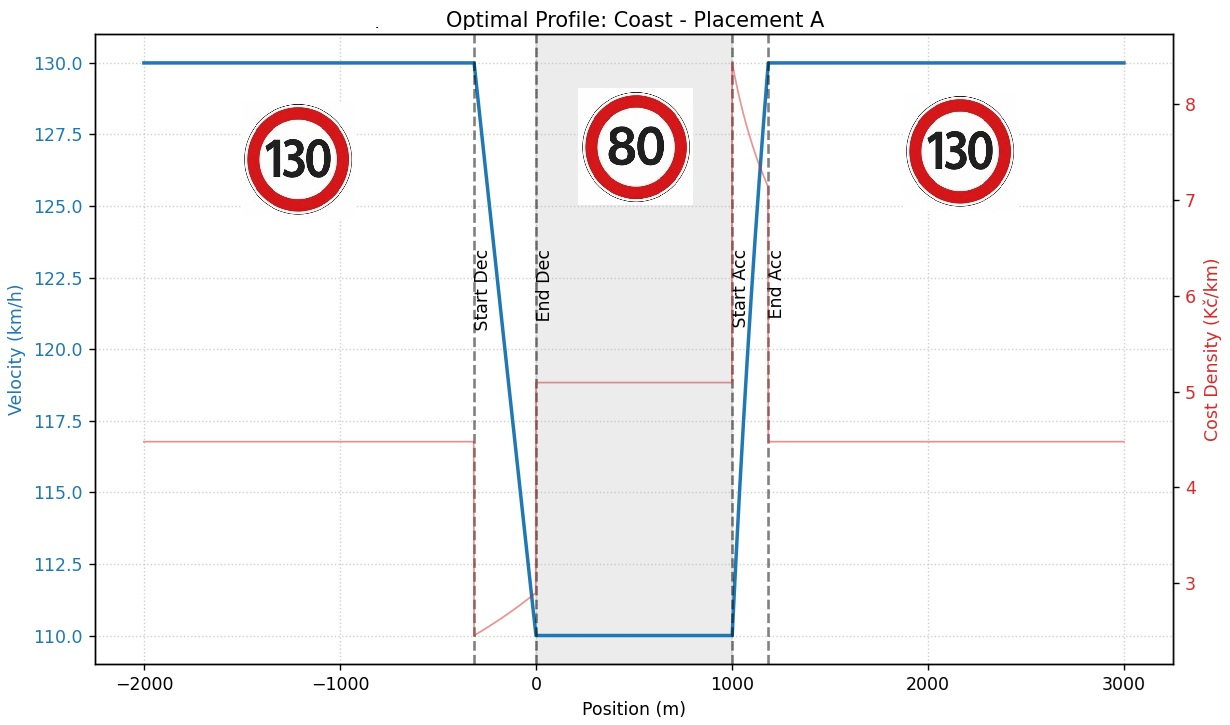
\includegraphics[width=\textwidth]{carArticle002.jpg}
\caption{Optimal speed profile and cost-density regime for the coasting deceleration variant resulting from the finite-dimensional optimization.
The shaded region indicates the reduced-limit zone $x\in[0,L]$ with $L=1000\,\mathrm{m}$.
Numerical parameters used in the code:
Dynamics (calibrated): $A=58.39\,\mathrm{m/s^2}$, $B=1.4726\times 10^{-4}\,\mathrm{m^{-1}}$, $\mu=5.8166\times 10^{-3}\,\mathrm{s^{-1}}$, $\mu_0=0.24793\,\mathrm{m/s^2}$, $v_0=1\,\mathrm{m/s}$, and physical braking $a=7\,\mathrm{m/s^2}$.
Costs: Time cost $C_t =300\,\mathrm{K\check{c}/h}$, fuel price $c_f=32\,\mathrm{K\check{c}/L}$.
Fuel model: $\gamma_u=19\,\mathrm{L/h}$ and $\gamma_0=0.6\,\mathrm{L/h}$.
Speed-limit regimes: $v_{\mathrm{lim},1}=130\,\mathrm{km/h}$ (outside), $v_{\mathrm{lim},2}=80\,\mathrm{km/h}$ (inside), with thresholds $v_{\max,1}=160\,\mathrm{km/h}$ and $v_{\max,2}=110\,\mathrm{km/h}$.
Expected-fine parameters: $p_L=1$, $P_{\mathrm{low}}=2500\,\mathrm{K\check{c}}$, $P_{\mathrm{high}}=15000\,\mathrm{K\check{c}}$.
Crucially, the enforcement intensity is modeled temporally as $\lambda=0.026\,\mathrm{h^{-1}}$ (approx.\ 1 check per 38 hours of driving), resulting in a constant fine rate (money/time) whenever $v > v_{\mathrm{lim}}$.}
  \label{fig:opt_profile_coast_A}
\end{figure*}

\section{Conclusion}
We reduced a continuous-time optimal driving problem with regime-dependent expected speeding fines to a finite-dimensional comparison within a PMP-motivated five-stage trajectory family.
The PMP implies bang--bang propulsion/braking with possible throttle-singular cruise arcs; this motivates the trajectory Ansatz.
We introduced a constant parasitic resistance term $\mu_0$ and showed how it can be calibrated together with drag and rolling coefficients from sparse fuel-consumption and coasting-deceleration measurements, yielding a smooth fuel-consumption curve consistent with data.
Within the five-stage family, deceleration and acceleration segments admit explicit quadratures for their distances and costs, and the relative placement of these arcs with respect to the reduced-limit zone produces four discrete placement options with closed-form total-cost expressions.

\end{document}
